\documentclass[a4paper, 11pt]{article}
\usepackage{listings}
\usepackage{xcolor}
%\usepackage[top=1.8cm, bottom=2cm, left=2cm, right=2cm]{geometry}
\usepackage{enumitem}
\usepackage{hyperref}

\usepackage{titlesec}

\usepackage{lmodern}

\usepackage{booktabs}


\usepackage{titling}
%\setlength{\droptitle}{-1.8cm}

\usepackage[bottom]{footmisc} %for moving footnotes down

\usepackage[british]{babel} %for word breaking at the end of lines

\usepackage{subfig}
\usepackage{graphicx}

\usepackage{wrapfig}

\usepackage{algorithm}
%\usepackage{amsmath}
%\usepackage{algorithmic}

\usepackage{algpseudocode}

\usepackage{multicol}
\usepackage{amsmath}

\usepackage{etoolbox}
\usepackage{mwe}

\usepackage{tikz}

\usepackage{caption}
\usepackage{subcaption}

\usepackage{capt-of}

\usepackage{footnote}

% Permette le note a piè di pagina nelle tabelle
\makesavenoteenv{tabular}
\makesavenoteenv{minipage}

\usepackage{caption}

\captionsetup[figure]{font=footnotesize}  % Sets the font size of figure captions
\captionsetup[table]{font=footnotesize}  


% Definizione personalizzata di \figurename
\renewcommand{\figurename}{\footnotesize Figure}
\renewcommand{\tablename}{\footnotesize Table}



\title{Diagnosing Alzheimer’s disease from handwriting}
\author{Gabriele Giudici (530344), Gabriele Billi Ciani (615560)\\University of Pisa\\ Data Mining and Machine Learning Course}
\date{A.Y. 2023-2024}

\begin{document}

\maketitle

\tableofcontents

\section{Introduction}

Neurodegenerative disorders, such as Alzheimer's disease, are characterised by the progressive deterioration of cognitive and motor functions, severely impacting the quality of life of those affected. Alzheimer's disease, in particular, leads to a gradual decline in memory, judgement, and other cognitive abilities. One intriguing aspect of Alzheimer's is its effect on fine motor skills, including handwriting. Handwriting analysis offers a unique, non-invasive window into the early detection of these cognitive impairments because it requires intricate coordination between various brain regions involved in motor planning and execution. With the advent of machine learning techniques, it is now possible to analyse handwriting dynamics more systematically and accurately, making them a valuable tool in the early diagnosis and monitoring of Alzheimer's disease.

The data set used in this project was introduced and utilised by Cilia et al.~(2022) in their study titled ``Diagnosing Alzheimer’s disease from on-line handwriting: A novel data set and performance benchmarking'' \cite{Cilia2022}. This paper presents the DARWIN (Diagnosis AlzheimeR WITh haNdwriting) data set, which is designed to aid in the early diagnosis of Alzheimer’s disease through handwriting analysis.

The DARWIN data set, described in Section \ref{sec:DARWIN-data-set}, is designed to support the early diagnosis of Alzheimer's disease by analysing handwriting dynamics. Its primary aim is to serve as a comprehensive resource for evaluating handwriting-based diagnostic methods and to facilitate the development of machine learning approaches to distinguish between Alzheimer's patients and healthy individuals.

To evaluate the effectiveness of the data set in supporting the early diagnosis of Alzheimer's disease, we conducted a comprehensive analysis comparing the performance of four different classification models. These models were tested both individually and in ensembles, utilising the full set of 450 features as well as features derived from specific tasks within the data set. The analysis included exploring various strategies such as majority voting, selecting the most informative tasks, and applying feature reduction techniques to optimise the classifiers' performance. The framework of the analyses conducted is explained in greater detail in Section \ref{sec:framework}.

\subsection{The DARWIN Data Set} \label{sec:DARWIN-data-set}

As previously mentioned, the DARWIN data set is designed to support the early diagnosis of Alzheimer's disease through the analysis of handwriting dynamics. The data set comprises handwriting samples from a total of 174 participants, including 89 individuals diagnosed with Alzheimer's disease (AD) and 85 healthy controls. The data were meticulously collected using a series of 25 handwriting tasks, categorised into graphic, copy, memory, and dictation tasks. Each task was designed to capture various aspects of handwriting, with a total of 450 attributes extracted from the handwriting data.

The raw data consist of digital handwriting data, which include coordinates (x, y), pressure, and timestamps (such as time on air and time on paper) recorded during the execution of each task. From those raw data, 18 features were extracted from each of the 25 tasks (thus getting the $18 \times 25 = 450$ attributes). The 18 features are consistent across all tasks, but their importance may vary depending on the nature of each specific task\footnote{A comprehensive description of these 18 features can be found in \cite{Cilia2022}.}.

All features are numeric and the data set is free from missing values, ensuring completeness and reliability in the analysis. This high level of data integrity is indicative of the rigorous data collection methods employed, resulting in a data set that requires minimal preprocessing and is well-suited for direct application in data mining and machine learning tasks.

For further details on the data set, on its creation and the experimental protocol used for gathering data, please refer to the paper by Cilia et al.~\cite{Cilia2022} and to the repository available at \url{https://archive.ics.uci.edu/dataset/732/darwin}.

\subsection{Analytical Framework} \label{sec:framework}

In this study, we have employed four classification models—Decision Tree (DT), Random Forest (RF), K-Nearest Neighbours (K-NN), and Gaussian Naive Bayes (GNB)—to evaluate their performance in diagnosing Alzheimer's disease using the DARWIN data set. These classifiers were selected based on the fact that they were theoretically covered during our coursework; however, the framework established here can be readily extended to include additional classifiers, as demonstrated by Cilia et al.~\cite{Cilia2022}, who examined a total of nine different models.

Initially, we assessed the performance of the four classifiers using the complete data set with all 450 features, as outlined in Section \ref{sec:baseline}. This provided a baseline understanding of each classifier's effectiveness in distinguishing between Alzheimer's patients and healthy controls.

Subsequently, we conducted a more granular analysis by training and evaluating the classifiers on 25 distinct feature sets, each corresponding to a specific handwriting task (Section \ref{sec:task-by-task}). This approach resulted in the creation of 25 task-specific classifiers for each model. We then noticed the possibility of ranking tasks for each classifier based on their performance, with the aim of developing ensemble models using majority voting strategies, as described in the following paragraph.

The 25 task-specific classifiers described were utilised to form ensemble models through majority voting (Section \ref{sec:majority-voting}). For each classification model, we trained separate classifiers on each of the 25 tasks and combined their predictions on a test set via majority voting. This approach allowed us to assess whether combining predictions across tasks could enhance overall diagnostic accuracy.
    
Building on the results from the previous step, we explored whether performance could be enhanced by selecting a subset of the best-performing tasks (Section \ref{sec:task-reduction}). This task selection process aimed to optimise classifier performance by focusing on the most informative tasks.
    
As an alternative to the task reduction described in the previous step, which naturally involves discarding entire sets of features associated with the excluded tasks, we explored whether standard feature reduction methods—methods that do not consider the task-specific structure of the data—\allowbreak could similarly enhance the classifiers' performance metrics (Section \ref{sec:feature-reduction}). While we applied these standard feature reduction techniques, we recognised that task reduction offers a significant advantage: it not only simplifies the feature set but also reduces the number of tasks that patients need to perform, thereby streamlining future data collection and making it more efficient.
    
Finally, we outlined strategies that integrate feature reduction, task selection, and majority voting (Section \ref{sec:proposals}) . These strategies were conceptualised to combine the strengths of each method and provide a comprehensive approach to optimising classifier performance.

\subsection{Overview of the Literature Review and Comparative Analysis}
Our work builds upon the foundational paper by Cilia et al.~(2022) \cite{Cilia2022}, which was referenced at the outset. Much of our analysis follows the methodologies presented in their study. However, we have consistently maintained a critical perspective, rigorously comparing our findings with those reported by Cilia et al. At times, we opted for different approaches, which are explained throughout the text. Additionally, we conducted novel analyses beyond those included in their paper. 

Rather than dedicating a separate section to comparison at the end, we found it more effective to integrate these comparisons and critical analyses directly into the relevant sections of the text.

\section{Experimental results}
In the following sections, we provide a detailed account of the studies conducted, which were introduced earlier in Section \ref{sec:framework}. These analyses are presented comprehensively, with an emphasis on the methodologies employed and the outcomes obtained. 

The Jupyter notebooks developed for these analyses are integral to this report. Readers are encouraged to consult these notebooks for further exploration and a broader range of results.

\subsection{Classification on the Full Data Set} \label{sec:baseline}
Our initial analysis focused on evaluating the performance of the four selected classifiers—DT, RF, K-NN, and GNB—using the complete DARWIN feature set (all 450 features), as illustrated in Figure \ref{fig:immagine1}. This approach served as our baseline, providing a fundamental understanding of each classifier's capability to differentiate between Alzheimer's patients and healthy controls.

\begin{figure}[h!]
    \centering
    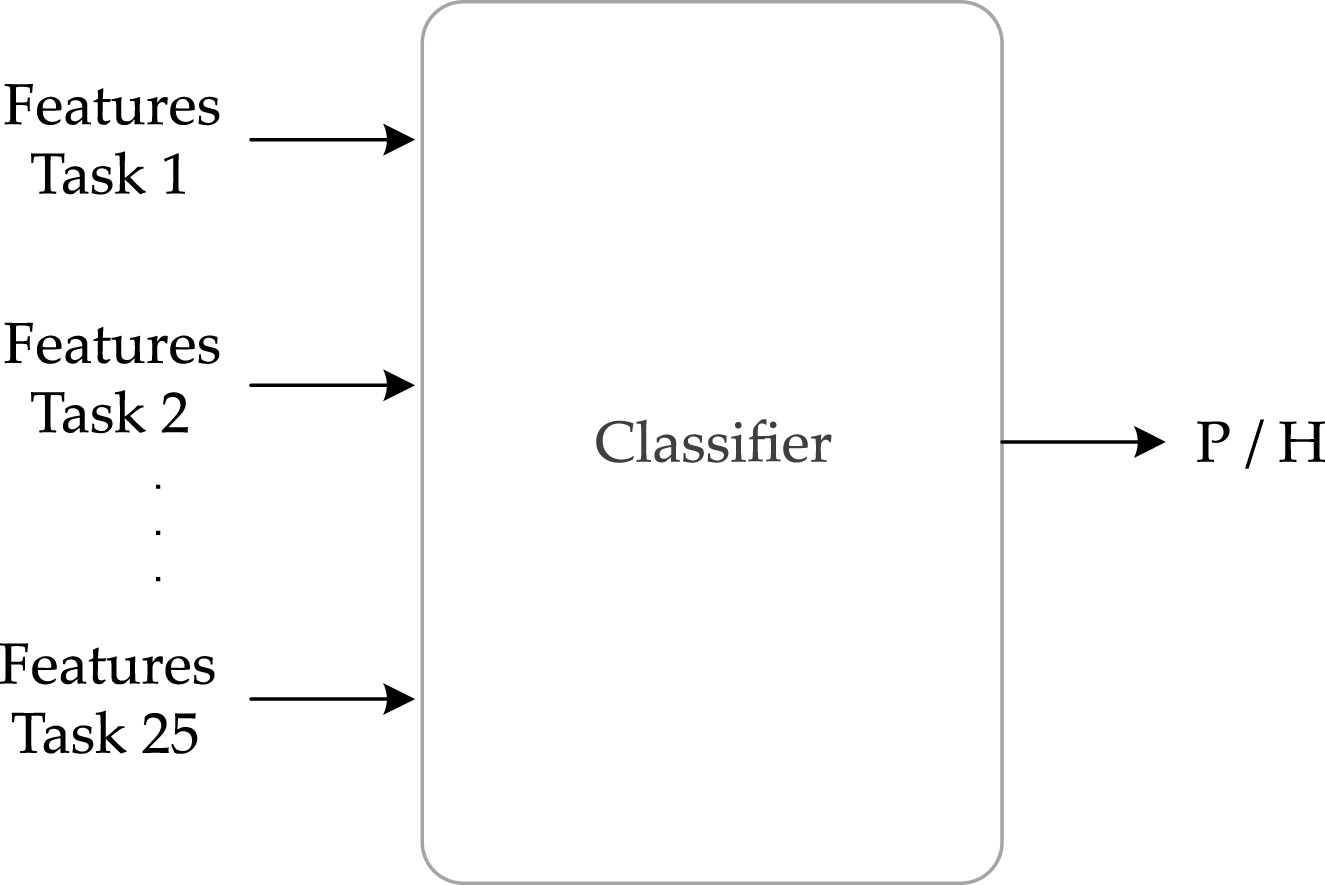
\includegraphics[width=0.5\textwidth]{Figures/immagine1.jpg}
    \caption{\footnotesize{Representation of classification performed combining all tasks' attributes (union of the features extracted from each of the 25 tasks). P=Patient, H=Healthy. From \cite{Cilia2022}.}}
    \label{fig:immagine1}
\end{figure}

Importantly, this baseline analysis did not leverage any knowledge of the data set's specific structure, particularly its composition of 25 distinct tasks. By using the full feature set without consideration of task divisions, we established a starting point from which to measure potential improvements in subsequent analyses: this initial evaluation allowed us to assess the raw predictive power of each classifier when presented with the entirety of the available data.

To optimise classifier performance, we utilised a grid search approach to identify the best hyperparameters for each model. Following this, we conducted k-fold cross-validation to obtain robust estimates of our performance metrics\footnote{Actually, in this analysis, we employed additional methodologies beyond k-fold cross-validation, which are discussed in more detail shortly, when we compare our metric collection approach with that of the reference paper by Cilia et al.}.

We employed standard performance metrics including accuracy, sensitivity (recall), specificity, precision and F-score ($F_1$) to gauge the effectiveness of each classifier. The detailed metrics can be found in Table \ref{table:baseline-metrics}.

\begin{table}[h!]
\centering
\scriptsize
\begin{tabular}{lcccc}
\toprule
\textbf{Model} & \textbf{Accuracy} & \textbf{$F_1$} & \textbf{Sensitivity} & \textbf{Specificity} \\
\midrule
DT & 0.8390 ± 0.0391 & 0.8497 ± 0.0404 & 0.9031 ± 0.0891 & 0.7839 ± 0.1020 \\
GNB & 0.8736 ± 0.0426 & 0.8825 ± 0.0335 & 0.9129 ± 0.0360 & 0.8322 ± 0.0639 \\
K-NN & 0.7190 ± 0.0985 & 0.6470 ± 0.1424 & 0.5262 ± 0.1574 & 0.9306 ± 0.0569 \\
RF & 0.8503 ± 0.0856 & 0.8571 ± 0.0785 & 0.9075 ± 0.0869 & 0.8098 ± 0.1687 \\
\bottomrule
\end{tabular}
\caption{\footnotesize Final aggregated performance metrics with 5-fold cross-validation for different models. All metrics are expressed as mean ± standard deviation.}
\label{table:baseline-metrics}
\end{table}

\vspace{-20pt}

\paragraph{Results Analysis and Comparison with Reference Study}
Comparing our results with the reference study (\cite{Cilia2022}), we found strong alignment between the two. All classifiers performed well, with their performance remaining robust against variations in the training and test samples. We also identified a group of top classifiers, which showed no statistically significant differences in mean accuracy and $F_1$ score.

The high sensitivities of these top classifiers confirm the reliability of the tasks included in the experiments in providing relevant information for distinguishing between AD patients and healthy individuals.

From a methodological standpoint, we highlight a difference between our approach and that of the reference study. Like Cilia et al., we performed a 5-fold cross-validated grid search to select the best hyperparameters for each classifier. However, while Cilia et al.~estimated the metrics by conducting twenty runs, each time randomly shuffling and splitting the dataset into training and test sets, we preferred to use k-fold cross-validation from the outset. This choice was made because we planned to use pipelines optimised specifically for k-fold cross-validation in later analyses. Nevertheless, for this baseline comparison, we also performed twenty iterations and demonstrated that there were no statistically significant differences between the metrics obtained using the two methods.

The results of this baseline analysis set the stage for our subsequent investigations, where we anticipated progressive improvements by incorporating task-specific knowledge and applying various feature selection and ensemble methods.

\subsection{Task-Specific Classification} \label{sec:task-by-task}
Building upon our baseline evaluation, we conducted a more detailed analysis to explore the diagnostic potential of individual handwriting tasks. This approach involved training and evaluating our four classifiers on 25 distinct feature sets, each corresponding to a specific handwriting task in the DARWIN data set.

This task-specific analysis resulted in the creation of 100 distinct classifiers: 25 task-specific classifiers for each of our four models\footnote{Also in this case, we performed a 5-fold cross-validated grid search to select the best hyperparameters for each classifier.}. We assessed the performance of these classifiers across all tasks, using the same metrics as in our baseline analysis. 

Due to space constraints, detailed metrics about this task-specific classification are not included in this report\footnote{Readers are encouraged to consult the Jupyter notebooks, which are an integral part of this work, for a comprehensive view.}; however, comments on these metrics can be found later in this section, during the comparison with the reference paper. 

\begin{figure}[h!]
    \centering
    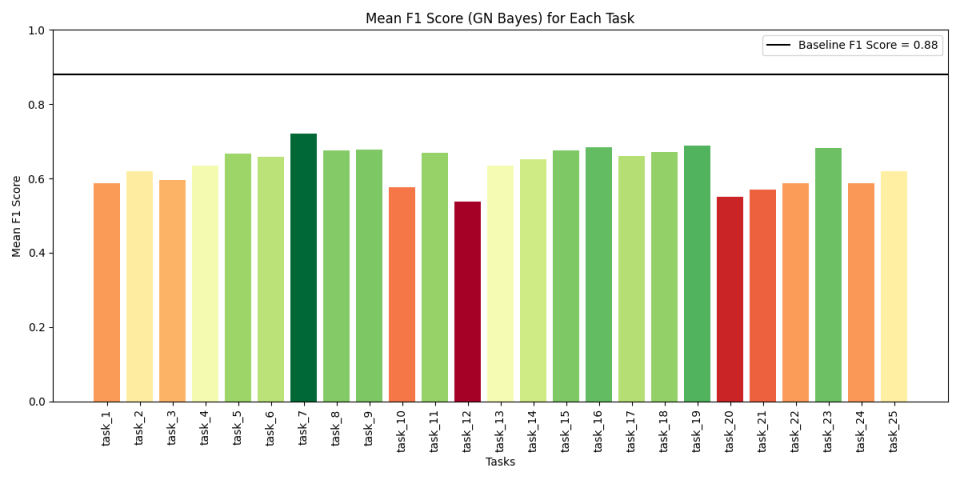
\includegraphics[width=\textwidth]{Figures/task-by-task.png}
    \caption{\footnotesize{Average $F_1$ score obtained by training and testing GNB on each task separately, compared with the average $F_1$ score of the GNB baseline model (using all tasks together).}}
    \label{fig:task-by-task}
\end{figure}

\paragraph{Results Analysis and Comparison with Reference Study}
Our results are consistent with the findings of the referenced study in several significant respects. We observed that, irrespective of the classifier employed, the metrics achieved on individual tasks were consistently lower than that attained in the baseline experiment (cf. Figure \ref{fig:task-by-task}). Even the top-performing models from the prior experiment exhibited reduced performance when applied to single tasks.

Furthermore, our analysis confirms that no single classifier outperformed all others across every task. Instead, each task was best addressed by a specific subset of models, which reinforces the idea that different tasks capture distinct aspects of handwriting movements. This variability underscores the importance of incorporating multiple tasks to achieve a more comprehensive understanding of these movements, rather than relying on any single task.

This analysis provides insight into which tasks each classifier performs best on, and conversely, which classifiers excel on each task. This intuition paves the way for more complex analyses, which we develop later and describe in the following sections.

\subsection{Ensemble Modelling via Majority Voting} \label{sec:majority-voting}

Building upon our task-specific analysis, we explored the potential of ensemble models using majority voting strategies. This approach aimed to leverage the strengths of individual task-specific classifiers to enhance overall diagnostic effectiveness. 

For each of our four classification models, we created an ensemble by combining the predictions of all 25 task-specific classifiers. This resulted in four model-specific ensembles, each integrating information from all handwriting tasks within a single classification framework. The final prediction for each test sample was determined by a majority vote among the constituent classifiers, as represented in Figure \ref{fig:immagine2}. 

\begin{figure}[h!]
    \centering
    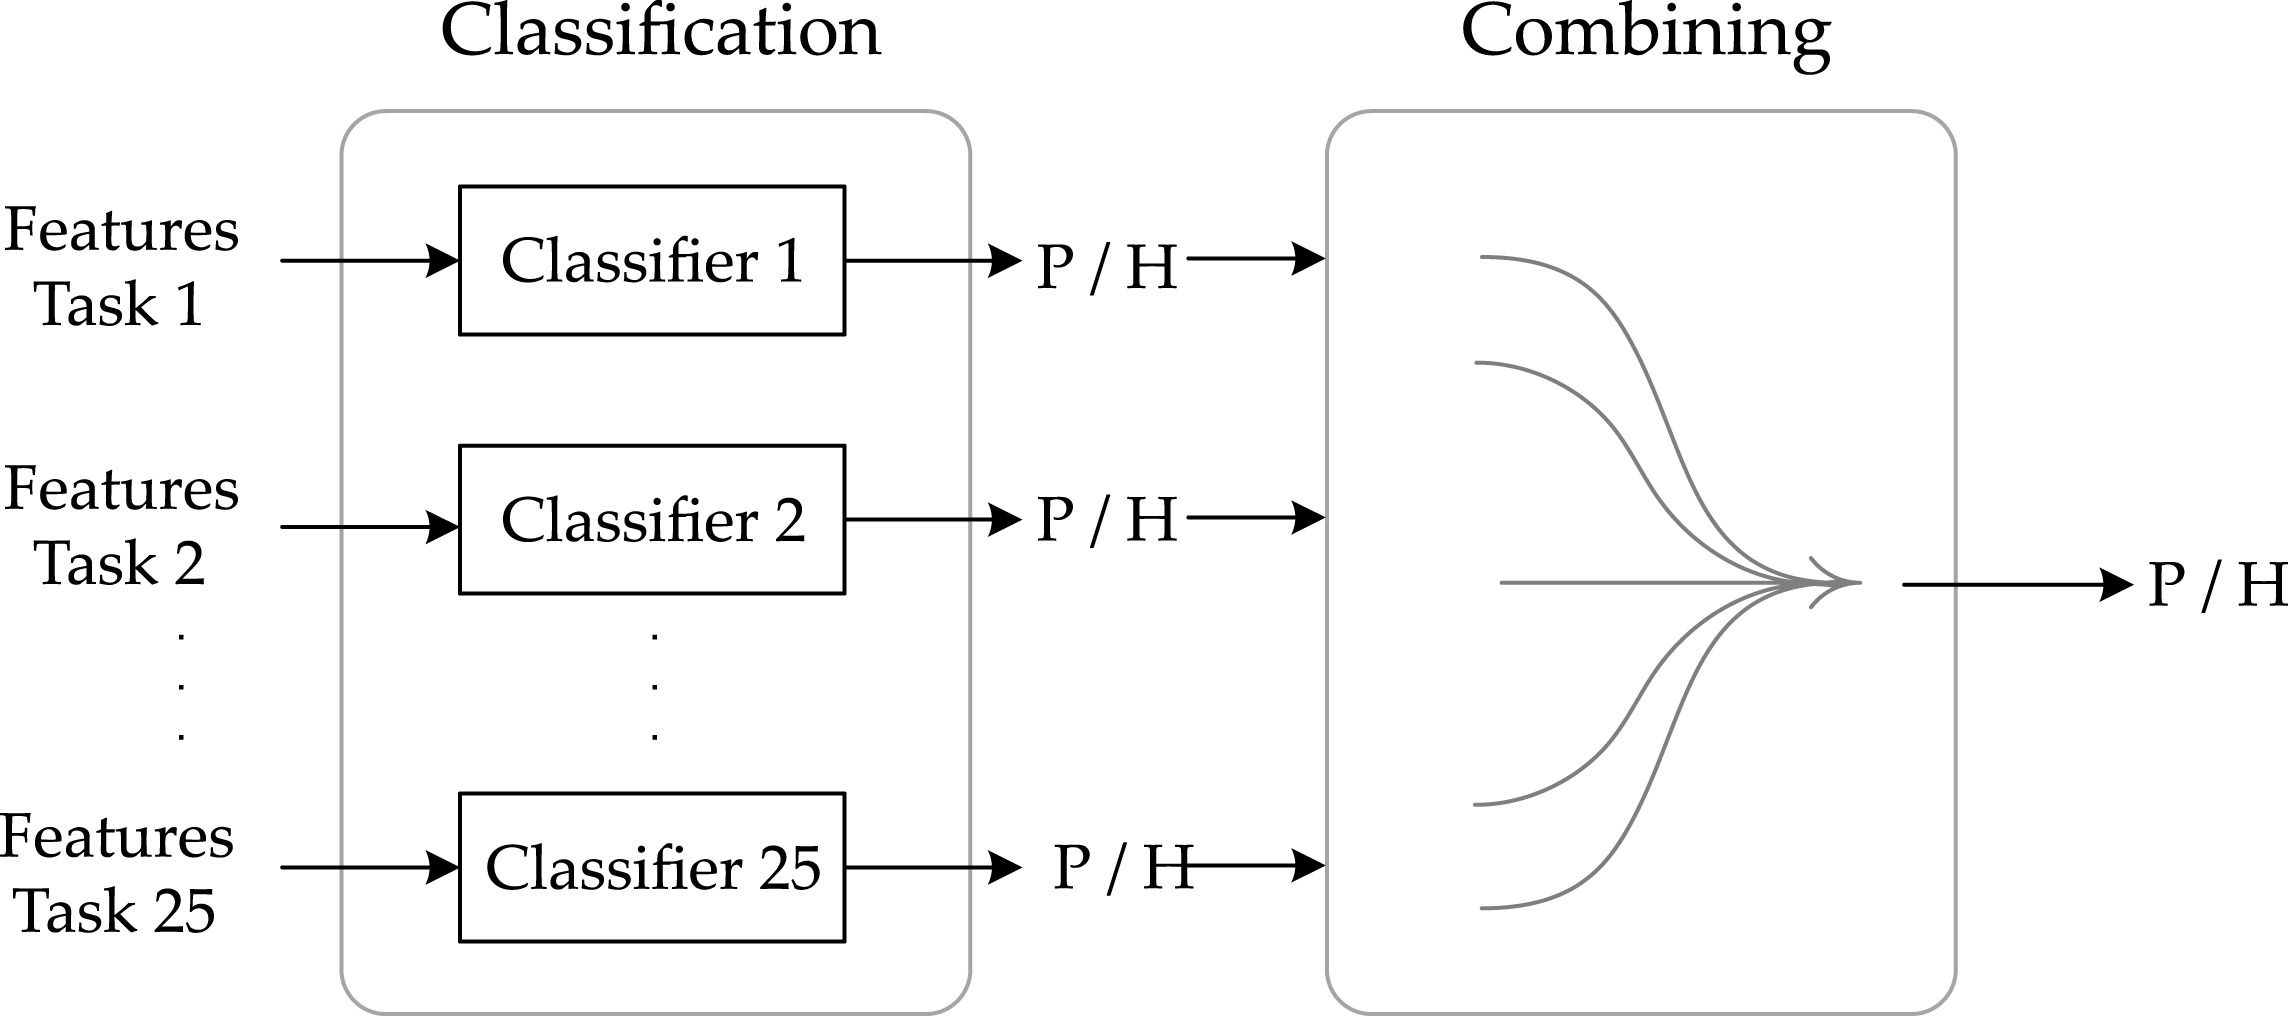
\includegraphics[width=0.8\textwidth]{Figures/immagine2.jpg}
    \caption{\footnotesize{Representation of classification achieved by training a separate classifier for each task and then combining their outputs using majority voting. P=Patient, H=Healthy. From \cite{Cilia2022}.}}
    \label{fig:immagine2}
\end{figure}

This methodology enabled us to assess that combining predictions across tasks can enhance overall diagnostic effectiveness compared to individual task-specific classifiers and to the baseline full-feature model. Indeed, we evaluated these ensemble models using the same performance metrics as in previous analyses and the results, presented in Table \ref{table:majority-voting}, provide insights into the effectiveness of these ensemble strategies.

\begin{table}[h!]
\centering
\scriptsize
\begin{tabular}{lcccc}
\toprule
\textbf{Model} & \textbf{Accuracy} & \textbf{$F_1$} & \textbf{Sensitivity} & \textbf{Specificity} \\
\midrule
DT & 0.8229 & 0.8409 & 0.9529 & 0.7000 \\
GNB & 0.7671 & 0.8019 & 0.9529 & 0.5917 \\
K-NN & 0.8414 & 0.8470 & 0.8941 & 0.7917 \\
RF & 0.8729 & 0.8747 & 0.9176 & 0.8306 \\
\bottomrule
\end{tabular}
\caption{\footnotesize Average metrics for different models achieved by using the majority voting strategy.}
\label{table:majority-voting}
\end{table}

\vspace{-15pt}

\paragraph{Results Analysis and Comparison with Reference Study}
In our analysis, in agreement with Cilia et al., we observed that all multi-classifiers demonstrated great performance, proving that different tasks capture different facets of handwriting and that the combined tasks effectively characterise the distinct aspects of AD patients and healthy individuals more accurately than any single task alone.

Consistent with the findings of Cilia et al., RF and K-NN outperformed the corresponding baseline classifiers in terms of overall accuracy and $F_1$ score, whereas GNB exhibited poorer performance. However, we were unable to replicate the substantial performance improvement observed for DT in their study, which reported accuracy of 94.29\%, specificity of 94.12\%, and sensitivity of 94.44\%.

\subsection{Task Reduction} \label{sec:task-reduction}
Building upon our findings from the ensemble models, we sought to refine our approach by investigating whether focusing on a subset of the most informative tasks could further enhance classifier performance. 

Our process involved the following steps: \begin{enumerate} \item Starting from the idea presented in Section \ref{sec:task-by-task}, we obtained the ranking of tasks based on their performance metrics for each classifier\footnote{The evaluation of the ranks was conducted exclusively on a training set to avoid a subtle form of data leakage. Using the same data for both rank and subsequent testing could artificially inflate the performance metrics.}. \item We created subsets of tasks, starting with the top-ranked ones and progressively adding tasks in order of their ranking. This is represented in Figure \ref{fig:immagine3}. \item For each subset, we evaluated a new ensemble model using the majority voting strategy described in Section \ref{sec:majority-voting}, obtaining curves such as the one shown in Figure \ref{fig:knn}. \end{enumerate}

%%%%%%%%%%%%%%%%%%%%%%

\begin{figure}[h!]
\centering

\begin{minipage}{0.3\textwidth}
    \centering
    \textbf{Original Tasks} \\[1em]
    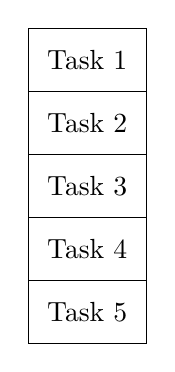
\begin{tikzpicture}[scale=0.8]
        \foreach \i in {1,...,5} {
            \node[draw, rectangle, minimum width=1.5cm, minimum height=0.8cm] at (0, -\i) {Task \i};
        }
    \end{tikzpicture}
\end{minipage}\hfill
\begin{minipage}{0.3\textwidth}
    \centering
    \textbf{Ranked Tasks} \\[1em]
    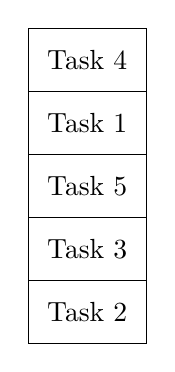
\begin{tikzpicture}[scale=0.8]
        \node[draw, rectangle, minimum width=1.5cm, minimum height=0.8cm] at (0, 0) {Task 4};
        \node[draw, rectangle, minimum width=1.5cm, minimum height=0.8cm] at (0, -1) {Task 1};
        \node[draw, rectangle, minimum width=1.5cm, minimum height=0.8cm] at (0, -2) {Task 5};
        \node[draw, rectangle, minimum width=1.5cm, minimum height=0.8cm] at (0, -3) {Task 3};
        \node[draw, rectangle, minimum width=1.5cm, minimum height=0.8cm] at (0, -4) {Task 2};
    \end{tikzpicture}
\end{minipage}\hfill
\begin{minipage}{0.3\textwidth}
    \centering
    \textbf{Task Subsets} \\[1em]
    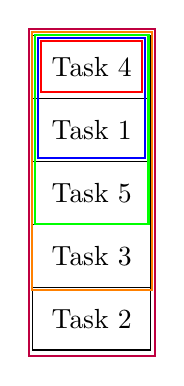
\begin{tikzpicture}[scale=0.8]
        \node[draw, rectangle, minimum width=1.5cm, minimum height=0.8cm] at (0, -2) {Task 4};
        \node[draw, rectangle, minimum width=1.5cm, minimum height=0.8cm] at (0, -3) {Task 1};
        \node[draw, rectangle, minimum width=1.5cm, minimum height=0.8cm] at (0, -4) {Task 5};
        \node[draw, rectangle, minimum width=1.5cm, minimum height=0.8cm] at (0, -5) {Task 3};
        \node[draw, rectangle, minimum width=1.5cm, minimum height=0.8cm] at (0, -6) {Task 2};
        
        \draw[red, thick] (-0.8,-1.6) rectangle (0.8,-2.4);
        \draw[blue, thick] (-0.85,-1.55) rectangle (0.85,-3.45);
        \draw[green, thick] (-0.9,-1.5) rectangle (0.9,-4.5);
        \draw[orange, thick] (-0.95,-1.45) rectangle (0.95,-5.55);
        \draw[purple, thick] (-1,-1.4) rectangle (1,-6.6);
    \end{tikzpicture}
\end{minipage}
\caption{Process of task ranking and subset creation. Each coloured rectangle represents a subset. The figure includes just 5 tasks (instead of 25) for illustration purposes.}
\label{fig:immagine3}
\end{figure}
%%%%%%%%%%%%%%%%%%%%%

These findings provide insights into which handwriting tasks are most crucial, for each of the classifiers tested, for accurate Alzheimer's disease diagnosis and how many tasks are necessary to achieve optimal performance.

%%%% DA CAMBIARE!!!!
%\begin{table}[h!]
%\centering
%\scriptsize
%\begin{tabular}{lccccc}
%\toprule
%\textbf{Model} & \textbf{Selected Tasks} & \textbf{Accuracy} & \textbf{$F_1$} & \textbf{Sensitivity} & \textbf{Specificity} \\
%\midrule
%DT & 4 & 0.8986 & 0.9007 & 0.9353 & 0.8639 \\
%GNB & 2 & 0.8671 & 0.8716 & 0.9176 & 0.8194 \\
%K-NN & 8 & 0.9157 & 0.9133 & 0.9088 & 0.9222 \\
%RF & 12 & 0.9114 & 0.9110 & 0.9265 & 0.8972 \\
%\bottomrule
%\end{tabular}
%\caption{\footnotesize Performance metrics for different models based on the number of selected tasks. Standard deviations are not reported due to low variability.}
%\label{table:selected_tasks_metrics}
%\end{table}
%\refstepcounter{footnote}
%\footnotetext[\thefootnote]{\label{fig:footnote}Additionally, it is important to note that the process of identifying the optimal number of tasks is subject to variability upon repeated executions of the code. This occurs because certain classifiers, such as RF, exhibit multiple points on the performance curve where the $F_1$ score reaches its maximum, with no statistically significant differences between them. As a result, the optimal number of tasks identified may differ slightly between iterations. Given that task reduction can streamline future data collection by reducing the number of tasks patients need to perform, it would be worthwhile to conduct a more detailed analysis of the performance curves. This could ensure the identification of the minimal yet most effective number of tasks.}

%\vspace{-15pt}

\paragraph{Results Analysis and Comparison with Reference Study}
For none of the models discussed in the previous section (cf. \ref{sec:majority-voting}), did we find a subset of tasks that, when used in an ensemble, led to improved performance compared to using all tasks. This contrasts with the findings of Cilia et al.; however, in our view, task reduction could still be considered in the following manner: through statistical analysis, it may be possible to identify subsets of tasks whose use in the ensemble results in performance that is not statistically different from that achieved by using all tasks. This approach would allow for the same high performance as previously observed, while offering the advantage of requiring each patient to undergo fewer tests. This intuition can be observed in Figure \ref{fig:knn}.


\begin{figure}[h!]
    \centering
    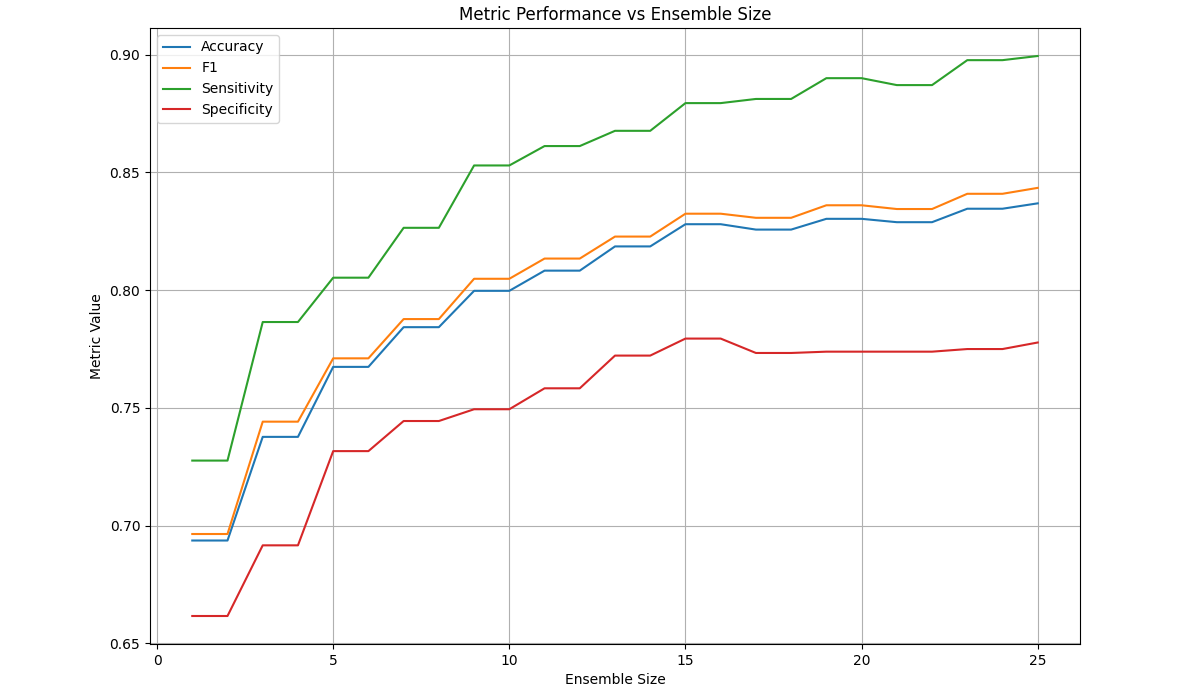
\includegraphics[width=\textwidth]{Figures/knn.png}
    \caption{\footnotesize{\textbf{K-NN} performance metrics for all subsets of tasks. Analogous images for the other models can be found in the Jupyter notebooks. Notice that with an ensemble size of 15, we already achieve performance comparable to that obtained using all tasks. As previously mentioned, it would be valuable to extend this approach through a more rigorous statistical analysis, potentially identifying smaller subsets of tasks that maintain equivalent performance.}}
    \label{fig:knn}
\end{figure}

%\vspace{-20pt}

It is important to emphasise again that this task selection process not only aims to optimise classifier performance but also has practical implications for future data collection. By identifying the most informative tasks, it is possible to potentially streamline the diagnostic process, thereby reducing the time and effort required from patients while maintaining high diagnostic accuracy. 

Cilia et al.~attempted to merge the features extracted from the subset of tasks yielding the best performance into a single feature vector, which was then used to train and test each model. However, this approach did not result in performance improvements compared to combining the outputs of task-specific classifiers. This further emphasizes the contribution of each task when considered individually, reinforcing the relevance of the task-by-task analysis. Instead of pursuing feature merging, we focused on feature reduction as further analysis, which was not explored in their work.

\subsection{Feature Reduction} \label{sec:feature-reduction}
In addition to task reduction, we explored standard feature reduction methods to potentially enhance classifier performance. Such analysis was not carried out by Cilia et al.~in the reference paper. Unlike task reduction, which simplifies the feature set by focusing on the most informative tasks, the feature reduction  analysis we have applied aims to reduce the dimensionality of the feature set without considering the task-specific structure. We applied Principal Component Analysis (PCA), Recursive Feature Elimination (RFE), Normalised Mutual Information Feature Selection (NMIFS) and  minimum Redundancy-Maximum Relevance (mRMR) to achieve this.

Although it is generally recommended to perform a grid search to find the optimal parameters for the classifier each time a subset of features is selected, for computational reasons, we did not re-conduct this search. Instead, we assumed that the parameters determined during the baseline analysis were valid for the reduced feature sets.

For each method, we followed a consistent pipeline approach: 
\begin{itemize}
    \item \textit{Data Preparation}: The data set was preprocessed to include only the relevant features, ensuring that non-feature columns were excluded (the ID column). In some cases, data normalisation was required.
    \item \textit{Feature Reduction}: Each technique was employed to reduce the feature set according to its specific criteria and constraints.
    \item \textit{Classifier Evaluation}: The performance of each classifier was assessed using cross-validation for evaluating the metrics.
\end{itemize}

The performance metrics were compared to those obtained from the full feature set and task reduction methods. 

The baseline serves as a crucial reference point in this feature reduction analysis from the entire parameter set. We anticipate that the task-specific feature reduction approaches proposed in Section \ref{sec:proposals} will be considerably more effective. Nonetheless, these results provide preliminary insights into which models and feature reduction strategies may offer greater efficacy.

Regarding PCA, we explored a range of variance thresholds for the retained principal components, spanning from 35\% to 98\%. This investigation was conducted across all four classifiers utilised in our analyses, focusing on the $F_1$ metric. The results indicate that for the GNB classifier, no threshold significantly improved (or even approached) the performance of the baseline analysis. For the DT classifier, we achieved results comparable to the baseline analysis with a variance threshold of 35\%. However, our initial hypothesis that the parameters used in the baseline model would remain optimal was not supported. We consistently obtained the same results across all thresholds until we adjusted the parameters, which led to improved performance. For K-NN, we observed that with a variance threshold of 35\%, the average $F_1$ score reached 0.7478, which was an improvement over the baseline $F_1$ score of 0.6470, although it still fell short of the $F_1$ scores obtained from majority voting analyses and task reduction approaches. Lastly, for RF, PCA did not surpass the performance of the baseline model.

Regarding NMIFS, we applied the pipeline exclusively to the RF model due to high computational demands. We were able to obtain results for a range of selected components from 2 to 50. Unlike PCA, NMIFS operates directly within the original feature set, allowing us to precisely identify which components are selected. With greater computational power, it would be feasible to determine which features are generally less informative and to integrate these findings with task reduction strategies. The results indicate a trend where all metrics improve as the number of features included increases, suggesting that exploring higher values of  selected features could be fruitful. However, due to the mentioned computational constraints, we were unable to fully investigate this possibility.

Also in the case of RFE the computational time proved to be extensive, allowing us to gather results only for the RF model\footnote{Due to its reliance on model-specific feature ranking, RFE could be practically applied only to the RF and DT models in our study.}. We evaluated the performance of RF with the number of selected features ranging from 5 to 450. All metrics reached their peak at 450 features, suggesting that feature reduction over the entire feature set with RFE does not seem to offer significant benefits.

The mRMR method, like NMIFS, selects features one by one up to a specified number, maximising their relevance to the target variable while minimising redundancy among the selected features. This ensures that each chosen feature adds unique and informative value. Moreover, it allows this analysis to be conducted in significantly less time compared to NMIFS, enabling us to complete all analyses efficiently. For this reason, we included mRMR in our feature reduction analysis. With it, we were able to gather results for all four classifiers, with the number of selected features ranging from 1 to 450. For the RF model, comparable results to the baseline analysis were observed only with a large number of features (over 300), revealing a similar trend to the one noted with RFE. In contrast, the DT model did not exhibit any feature subset size smaller than the maximum that led to performance improvements over the baseline. The K-NN classifier showed a performance peak with between 15 and 60 features (cf. Figure \ref{fig:mrmr-knn}), surpassing by far the baseline results\footnote{As previously mentioned, we have used in this analysis the same parameters found with the grid search before the baseline analysis, where the optimal value of \( k \) for the K-NN classifier was found to be 1. It is highly likely that operating with 450 features, given the high dimensionality, impaired the model’s ability to accurately identify the nearest neighbour for the classification task. This explains why reducing the number of features led to a significant improvement in the model’s performance.}. The GNB model indicated that performance reached baseline levels with approximately 70 selected features, with no further improvement observed as the number of features increased (cf. Figure \ref{fig:mrmr-gnb}).

\begin{figure}[h!]
    \centering
    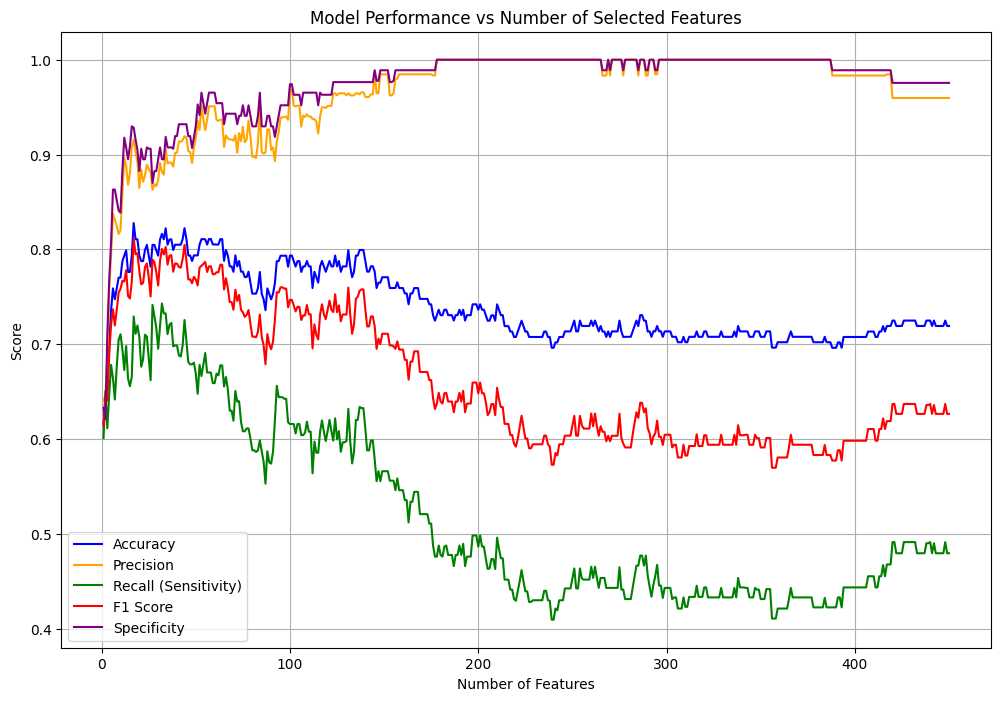
\includegraphics[width=\textwidth]{Figures/mrmr-knn.png}
    \caption{\footnotesize{Performance trends of the \textbf{K-NN} classifier as the number of selected features increases, showing that a peak in performance is reached with approximately 15-60 features, with a significant decrease beyond that point.}}
    \label{fig:mrmr-knn}
\end{figure}

\begin{figure}[h!]
    \centering
    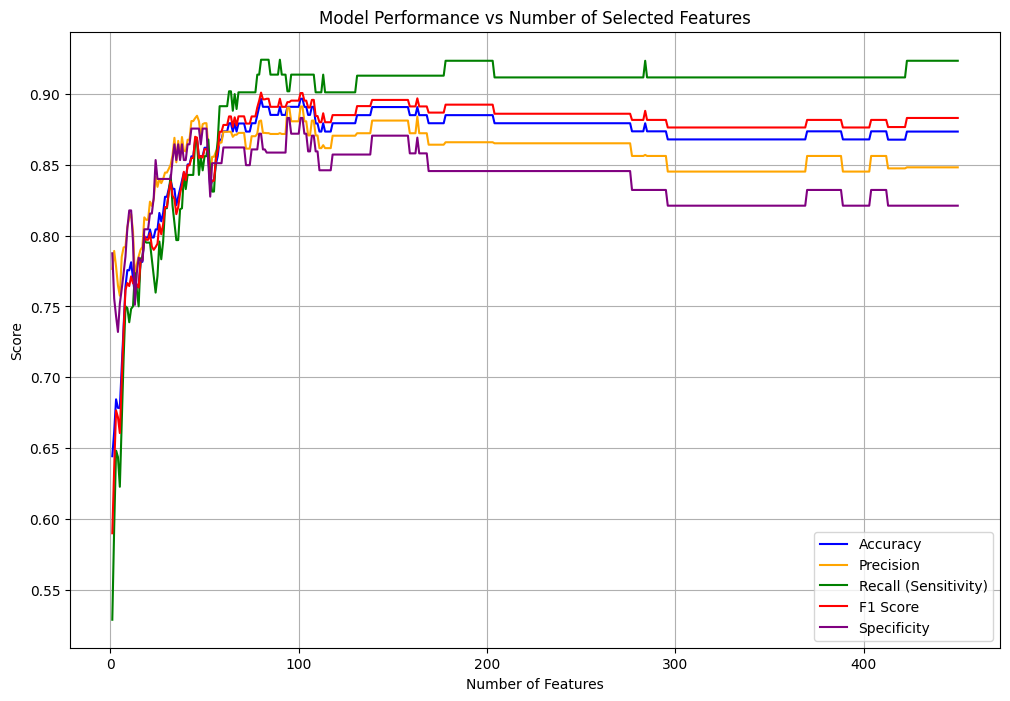
\includegraphics[width=\textwidth]{Figures/mrmr-gnb.png}
    \caption{\footnotesize{Performance trends of the \textbf{GNB} classifier as the number of selected features increases, showing that baseline performance is reached with approximately 70 features, with no significant improvement beyond that point.}}
    \label{fig:mrmr-gnb}
\end{figure}

As previously mentioned, we did not expect, with this feature reduction analysis, to surpass the results achieved in the previous sections. Rather, our aim was to open avenues for new types of analysis. In the subsequent section, we will present additional approaches and methodologies to feature reduction that may offer more effective solutions for simplifying and enhancing model performance.

\section{Proposed Enhancements and Future Experiments} \label{sec:proposals}

Based on our current findings, we propose a couple enhancements and future experiments to further optimise the diagnostic performance of handwriting analysis for Alzheimer's disease. Our proposed approaches focus on combining feature reduction with task reduction strategies, aiming to refine and streamline the classification process.

\paragraph{Reduction on Task-Specific Data}

One enhancement involves applying feature reduction techniques directly to each handwriting task before classification. This approach includes the following steps:
\begin{itemize}
    \item \textit{Task-Specific Feature Reduction}: Perform feature reduction methods on the features extracted from each individual task.
    \item \textit{Classifier Training}: Train classifiers on the reduced feature sets from each task.
    \item \textit{Ensemble Methods}: Create ensemble models by combining predictions from classifiers trained on feature-reduced tasks. This can be achieved through majority voting or other ensemble strategies to integrate the strengths of each task-specific classifier.
\end{itemize}

By applying feature reduction to each task, we aim to enhance the classifier's ability to discern subtle differences between Alzheimer's patients and healthy controls, potentially improving overall diagnostic accuracy.

\paragraph{Combining Task Reduction with Feature Reduction}

Another promising direction is to combine task reduction with feature reduction methods. This approach involves:
\begin{itemize}
    \item \textit{Task Reduction}: Identify and select a subset of the most informative tasks based on performance metrics from previous analyses.
    \item \textit{Feature Reduction on Selected Tasks}: Apply feature reduction techniques only to the features of the remaining tasks after task reduction.
    \item \textit{Classifier Training and Evaluation}: Train classifiers using the reduced feature sets from the selected tasks and evaluate their performance, even by using ensemble strategies. 
\end{itemize}

This hybrid approach leverages the benefits of both task and feature reduction, aiming to streamline the diagnostic process while maintaining high accuracy.

\paragraph{Task Reduction with Redundancy Analysis}
Another intriguing aspect to explore is performing task reduction (as done in Section \ref{sec:task-reduction}) with an additional consideration of redundancy analysis. Specifically, tasks should not only be added based on their rank but also by considering their correlation with the tasks already included in the subset used for the ensemble. If the new task to be included is highly correlated with the previous one, it might be more beneficial to skip it and instead select the next task with a lower correlation.

\section{Conclusions}
In this study, we explored various methodologies for enhancing the performance of classification models in diagnosing Alzheimer's disease using the DARWIN dataset. Our analysis encompassed a comprehensive baseline evaluation, task-specific assessments, ensemble modelling via majority voting, task reduction, and standard feature reduction techniques. We observed that each model benefited from different approaches; for instance, GNB performed optimally in the baseline analysis, while K-NN showed poor performance in the baseline but improved significantly with ensemble methods and feature reduction.
%We found that while ensemble methods could in some cases improve diagnostic accuracy, task reduction strategies offered a more streamlined approach, efficiently reducing the number of required tasks without compromising performance. Feature reduction techniques provided limited improvements compared to task-specific approaches but highlighted potential for further investigation. 

Overall, our findings underscore the importance of leveraging both task-specific (which could offer the advantage of requiring each patient to undergo fewer tests) and feature-specific strategies to optimise diagnostic performance.  Future research could benefit from integrating these approaches to refine and enhance early detection methods for Alzheimer's disease.

\begin{thebibliography}{99}
\bibitem{Cilia2022}
Cilia, N. D., De Gregorio, G., De Stefano, C., Fontanella, F., Marcelli, A., \& Parziale, A. (2022). Diagnosing Alzheimer’s disease from on-line handwriting: A novel data set and performance benchmarking. \textit{Engineering Applications of Artificial Intelligence}, 111, 104822. \url{https://doi.org/10.1016/j.engappai.2022.104822}
\end{thebibliography}



\end{document}